\chapter{Recursive distributional equations}
\label{ch:rde}

% Part V, added 2026-09-25 from ~/Downloads/chygraph_master_equation/draft.tex,
% Sec. 6 (probability). Secs. 1-4 rewrite equations the book already
% carries in the vocabulary of Aldous and Bandyopadhyay's recursive
% distributional equations and of the objective method; Sec. rde-computed
% runs both the linearised and the nonlinear test (statmech.endogeny,
% probe/endogeny.py, figs/endogeny.py). The relation between endogeny and
% replica symmetry breaking is in the literature (Aldous-Bandyopadhyay's
% open problems; Bandyopadhyay 2011), and carrying the perturbation with the
% field is the standard way of computing the RS stability line (Montanari-
% Ricci-Tersenghi 2003; Rivoire et al. 2004; Zdeborova-Krzakala 2007); what
% is new here is the Theorem 11(c) framing, the localisation of a failure to
% the interior operator, and the hitting-set application. Revised 2026-09-26
% after ~/Downloads/book_review.md.

The chygraph equation of Chapter~\ref{ch:chyequation} says that an unknown
law is reproduced by a random number of independent copies of itself, passed
through a random map. Probability has a name for an equation of that shape,
a survey of what is known about it, and two notions --- \emph{endogeny} and
\emph{bivariate uniqueness} --- that turn out to be the replica-symmetric
assumption and the de Almeida--Thouless test, said in a language where the
first is a property to be proved rather than an ansatz and the second is a
criterion rather than a stability calculation.

This chapter makes the identification equation by equation. The ensemble map
of Sec.~\ref{sec:substitution} and the pair of Sec.~\ref{sec:ce-equation}
are written in the form the probabilists use; the assumption each fixed
point carries is named; the affine case, which the book meets once, in
Chapter~\ref{ch:localization}, is matched to the smoothing transform; and
the random object the ensemble converges to locally is identified, with its
mean matrix, which is the threshold tensor of Chapter~\ref{ch:percolation}.
The chapter closes with what the book gets from this and what the field
could get back.

\section{The connection}
\label{sec:rde-connection}
\index{recursive distributional equation|textbf}
\index{population dynamics}

\citet{aldous2005} survey equations of the form
\begin{equation}
  X\ \stackrel{d}{=}\ g\bigl(\xi;\,X_{1},X_{2},\dots,X_{N}\bigr),
  \label{eq:rde-form}
\end{equation}
in which $X_{1},X_{2},\dots$ are independent copies of the unknown law, $N$
is a random number of them, $\xi$ is independent randomness carried by the
map, and $\stackrel{d}{=}$ asserts equality of laws. They call it a
\emph{recursive distributional equation}, and the survey's title names the
case they treat in most detail, in which $g$ is a maximum or a minimum. The
book has been solving equations of this form since Chapter~\ref{ch:statmech},
and its population dynamics is the standard numerical method for them: a
sample of the law, updated by drawing $N$ and $\xi$ and applying $g$, which
is what every population in Chapters~\ref{ch:hittingset}
to~\ref{ch:satisfiability} does.

\paragraph{The ensemble map is one of them.} Take Eq.~\eqref{eq:ensemblemap}
with a single container layer, so that the bracket is a single excess
function $\bar\Phi$. It says that $P$, the law of the field a node sends up
into a complex, satisfies
\begin{equation}
  h\ \stackrel{d}{=}\ B+\sum_{n=1}^{N}u_{n},
  \qquad N\sim\bar\Phi,\quad u_{n}\sim Q\ \text{independent},
  \label{eq:rde-up}
\end{equation}
and that $Q$, the law of what a complex emits, satisfies
\begin{equation}
  u\ \stackrel{d}{=}\ u\bigl(h_{1},\dots,h_{c-1}\bigr),
  \qquad c\sim\bar G,\quad h_{j}\sim P\ \text{independent},
  \label{eq:rde-down}
\end{equation}
with $u(\cdot)$ the emitted field of Eq.~\eqref{eq:emitted}. Substituting
the second into the first gives one equation of the form
\eqref{eq:rde-form} for $P$ alone, with $\xi=(N;c_{1},\dots,c_{N})$ the
counts, $g$ the composition of the two steps, and the copies of $X$ the
fields on the members of the $N$ complexes. The sum in Eq.~\eqref{eq:rde-up}
is what makes the ensemble version a convolution, exactly as
Sec.~\ref{sec:upstep} said, and the map $u(\cdot)$ is the whole of the
model.

\paragraph{The chygraph equation is a system of them.} With layers and
nesting, Eqs.~\eqref{eq:ensplus} and~\eqref{eq:ensminus} are one equation
of the form \eqref{eq:rde-form} for each directed inclusion type $(m,l,\pm)$,
$2L^{2}$ of them, coupled in the way Fig.~\ref{fig:themap} draws: the
unknown of type $(m,l,+)$ is built from copies of the unknowns of types
$(l,k,-)$, one per container of layer $k$ other than the one answered, and
of types $(l,k,+)$, one per member; the unknown of type $(m,l,-)$ from the
same two families with the excess on the other side. The randomness $\xi$
is the vector of counts, drawn from the four families of generating
functions of Sec.~\ref{sec:ensembles}, and $g$ is Eq.~\eqref{eq:chyop}. The
survey treats systems of this kind in passing, as a single equation on a
product space; the index set is what makes the chygraph version a system in
its own right, and Sec.~\ref{sec:rde-local} says what the index set is.

\paragraph{The split.} A general recursive distributional equation is one
opaque map $g$. The chygraph equation is not. Its $g$ is the composition of
two things of different character: a commutative step, the product over
containers, which is the exterior product $\otimes$ of Eq.~\eqref{eq:chyop}
and carries no model; and one nonlinear map of bounded arity, the interior
operator $\Tint_{l}$, which carries all of it and acts on at most $c_{l}$
arguments. Everything this chapter says beyond the survey follows from that
split. Table~\ref{tab:ce-substitutions} lists what the two steps are in each
of the book's calculations, and reading it as a table of recursive
distributional equations is reading it as the survey would: the first row
is degenerate, a point mass reproduced by a point mass; the second and
third are sum-type, with $g$ smooth; the hard-field rows of
Chapters~\ref{ch:hittingset} to~\ref{ch:satisfiability}, where a message is
an integer and the interior is a maximum or a minimum over forbidden
assignments, are the max-type equations the survey is about.

\section{Endogeny and replica symmetry}
\label{sec:rde-endogeny}
\index{endogeny|textbf}
\index{bivariate uniqueness|textbf}
\index{replica symmetry}
\index{de Almeida--Thouless line}

A solution of Eq.~\eqref{eq:rde-form} is a law. Behind it is a random
object: unroll the recursion and the copies $X_{1},\dots,X_{N}$ each have
their own copies, so that a solution lives on a random tree whose vertices
carry the innovations $\xi$, and the question the survey asks is whether the
value at the root is determined by that tree. A solution is
\emph{endogenous} when $X$ is a measurable function of the innovations
$\{\xi_{v}\}$ on the tree below it --- no randomness enters from infinity.
When it is not, the same tree of innovations supports many values at the
root, differing by something that is not visible at any finite depth.

That is the replica-symmetric assumption, stated as a property, and the
relation is not new: the survey raises it among its open problems, and
\citet{bandyopadhyay2011} works it out for the logistic equation. The
fixed point of Sec.~\ref{sec:substitution} carries one field per inclusion,
a function of the chygraph below the inclusion and of nothing else; that is
Sec.~\ref{sec:replicas}'s first assumption, that the message has one thing
to say, and it is endogeny. Its failure is where Sec.~\ref{sec:onestep}
begins: the space of solutions shatters into clusters, each cluster would
send its own field along the same inclusion, and the field at the root is
no longer fixed by the innovations below it but by which cluster the
boundary at infinity selects. The survey of Sec.~\ref{sec:onestep}, a law
over fields at fixed realisation, is the probabilist's non-endogenous
solution seen from the physics side.

\paragraph{The test.} What makes this more than a translation is that
endogeny has a computable criterion. Run two copies of the recursion on
the same tree of innovations, with the copies of the unknown drawn
independently at the leaves,
\begin{equation}
  (X,X')\ \stackrel{d}{=}\
  \Bigl(g(\xi;X_{1},\dots,X_{N}),\ g(\xi;X'_{1},\dots,X'_{N})\Bigr),
  \label{eq:rde-bivariate}
\end{equation}
the pairs $(X_{j},X'_{j})$ independent and identically distributed, and ask
whether the only solution whose margins are the given fixed point
is the one concentrated on the diagonal $X=X'$. \citet{aldous2005} call
this \emph{bivariate uniqueness}, and their Theorem~11 has three parts.
Endogeny implies bivariate uniqueness with no condition. The converse holds
when the bivariate map is weakly continuous. And, whether or not it is,
endogeny holds if and only if the iterates of the bivariate map started
from the product law $\mu\otimes\mu$ converge to the diagonal, which is
part~(c) of the theorem and the definition made computable: a population
dynamics with two entries per element, started independent, iterated, and
watched for whether it is driven to agree.

\paragraph{Where a failure can come from.} On a chygraph the split of
Sec.~\ref{sec:rde-connection} localises the answer. The commutative step
preserves the diagonal trivially: if every pair $(u_{n},u'_{n})$ agrees then
so does the pair of products, and conversely a difference in the product is
a sum of differences in the factors. So a failure of endogeny can come only
from the interior operator --- for the full map, not only its
linearisation, since the argument used nothing but the commutativity of the
relay --- and it is decided by how $\Tint_{l}$ transmits a difference
between its two arguments. Linearise Eq.~\eqref{eq:rde-bivariate}
about the diagonal, writing $D=X-X'$ for the difference on an inclusion.
Through the up step a difference is relayed unchanged, one factor of one
per container. Through the down step it is transmitted with the kernel
derivative,
\begin{equation}
  D_{a\to i}=\sum_{j\in\del a,\,j\ne i}
    \frac{\partial u}{\partial h_{j}}\Big|_{\mathrm{fp}}\,D_{j\to a}
  +O(D^{2}),
  \label{eq:rde-diff}
\end{equation}
one derivative per member leg, and $\hat u'$ on the own leg where there is
one. The differences on distinct legs are independent and of either sign,
so the quantity that propagates is the mean square: at the trivial fixed
point $\ave{D^{2}}$ is multiplied by $u'^{2}$ per member leg and by
$\ave{\sbar}$ legs per complex, which is Eq.~\eqref{eq:branch} with $u'$
replaced by $u'^{2}$. That is Sec.~\ref{sec:atline}'s de Almeida--Thouless
line, and the reweighting of Eq.~\eqref{eq:reweight} says that nothing else
in the tensor moves. The step that needs the trivial fixed point is the
factorisation of $\ave{u'^{2}D^{2}}$ into $\ave{u'^{2}}\ave{D^{2}}$: at a
non-trivial fixed point the perturbation is not independent of the field
it rides on, and Sec.~\ref{sec:rde-computed} measures what that costs.

So the de Almeida--Thouless tensor --- the $2L^{2}$ operator of
Sec.~\ref{sec:ce-yields} with $u'$ replaced by $u'^{2}$ --- \emph{is}
bivariate uniqueness for this class of equations, at the linear level. The
qualification matters and is stated as what it is. Linear stability of the
diagonal is necessary for endogeny: by part~(c) of the theorem, if the
diagonal is unstable the iterates from $\mu\otimes\mu$ cannot converge
to it, and bivariate uniqueness then fails through part~(b) when the map
is weakly continuous. Its loss, where the mean-square difference grows, is
an argument --- about second moments under the linearised map, where the
theorem's convergence is in law --- that the replica-symmetric fixed point
is not endogenous; it is not sufficient, because a pair started far from
the diagonal can fail to converge to it while every small perturbation
decays. Carrying the perturbation through the recursion in this way, as a
second entry alongside the field, is how the replica-symmetric stability
line has been computed on diluted models since \citet{montanari2003} and
\citet{rivoire2004}, and \citet{zdeborova2007} say explicitly that the
factorised average overstates stability; what the theorem adds is the
statement that the same computation decides endogeny. The nonlinear test, part~(c) of
the theorem run as two coupled populations, is done in
Sec.~\ref{sec:rde-computed} for two of the models of
Table~\ref{tab:ce-substitutions}, and on both the boundary it finds is the
linearised one, properly carried. What it decides is whether the de Almeida--Thouless line, which
Sec.~\ref{sec:atline} obtained from a local argument and
Chapter~\ref{ch:hittingset} used as a warning, is the whole boundary of
endogeny or only its local part; on the spin glass and the hitting set it
is the whole of it.

\section{The smoothing transform}
\label{sec:rde-smoothing}
\index{smoothing transform|textbf}
\index{mobility edge}

The linear case of Eq.~\eqref{eq:rde-form}, in which $g$ is affine in the
copies,
\begin{equation}
  X\ \stackrel{d}{=}\ \sum_{n=1}^{N}A_{n}X_{n}+C,
  \label{eq:rde-smoothing}
\end{equation}
with random non-negative weights $A_{n}$ and a random shift $C$, is the
\emph{smoothing transform}, and its fixed points are classified by
\citet{alsmeyer2012}. The classification is stated in terms of
$m(\beta)=\ave{\sum_{n}A_{n}^{\beta}}$, the growth rate of the $\beta$-th
moment of a product of weights along a branch, and its standing assumption
is a \emph{characteristic exponent}: a $\beta^{*}>0$ with
$m(\beta^{*})=1$ and $m>1$ below it. Since $m(0)=\ave{N}>1$, such an
exponent exists exactly when $m$ dips to one, $\min_{\beta}m(\beta)\le1$,
and then, provided $\beta^{*}\le1$, the homogeneous equation, $C=0$, has
non-degenerate non-negative fixed points, mixtures of $\beta^{*}$-stable
laws \citep{durrett1983,alsmeyer2012}; when $\min_{\beta}m(\beta)>1$ it has
none. The physical width, the imaginary part of the Green's function over
the absorber, solves the inhomogeneous equation with $C=|G_{i}|^{2}$, whose
fixed point is a perpetuity-type sum with a power-law tail of exponent
$\beta^{*}$ by the Kesten--Goldie mechanism; the homogeneous fixed points
are its scaling limit, not the object Chapter~\ref{ch:localization}
iterates.

The book meets an affine down step once. Chapter~\ref{ch:localization}'s
message is a resolvent, its interior is the Schur complement of
Eq.~\eqref{eq:schur}, and the localised phase is the fixed point at which
every message is real. The question of whether that fixed point is stable
is asked of the imaginary parts, with the real parts frozen at their
distribution, and Eq.~\eqref{eq:imlinear} is the answer: an imaginary part
is a sum over the other members of the imaginary parts they carry,
weighted by the positive random numbers $t^{2}v_{j}^{2}$. That is
Eq.~\eqref{eq:rde-smoothing} with $C=0$, $N$ the number of other members
across all containers, and $A_{n}$ the squared entries of the inverse
interior matrix. Section~\ref{sec:mobility} locates the mobility edge by
the growth rate $\lambda(\beta)$ of the $\beta$-th moment, at
$\min_{\beta}\lambda(\beta)=1$ \citep{abouchacra1973}. That
$\lambda(\beta)$ is $m(\beta)$, and the two sides of the edge are the two
sides of the classification, in an order that has to be stated because it
is the reverse of the naive one. On the localised side
$\min_{\beta}\lambda<1$, a characteristic exponent $\beta^{*}<1/2$ exists,
and the linearised equation has the non-degenerate fixed points of
\citeauthor{alsmeyer2012}: they are the laws of the widths scaled by the
absorber, heavy-tailed with exponent $\beta^{*}$, which is the known form
of the imaginary part of the Green's function in the localised phase of
the Bethe lattice \citep{abouchacra1973,mirlin1991}. On the extended side
$\min_{\beta}\lambda>1$, no exponent exists and the homogeneous linear
equation has no non-degenerate fixed point at all: the widths grow until
the nonlinear terms of the full recursion, Eq.~\eqref{eq:schur}, set them,
which is the physics of an extended state. The mobility edge is the
boundary case, $\min_{\beta}m(\beta)=1$ attained at the characteristic
exponent, and it is in that sense a statement about the fixed points of a
smoothing transform whose weights are Chapter~\ref{ch:localization}'s
Schur complements. The position of the minimum, $\beta=1/2$ on a tree by the symmetry of the kernel
\citep{mirlin1991}, is a property of the weights and not of the criterion,
which is why Sec.~\ref{sec:mobility} checks it on the ensembles with
triangles rather than assuming it.

Two remarks and no more. The de Almeida--Thouless line of the previous
section is a first-moment criterion at a fixed exponent and not a minimum
over $\beta$: the difference $D$ has random sign, so it is not a smoothing
transform on the non-negative cone, and what propagates is $D^{2}$ with
weights $u'^{2}$, whose condition is $m(1)=1$ for those weights.
Section~\ref{sec:mobility}'s ``a fractional power in place of the square''
is the comparison between that fixed exponent and the minimising one. And
the non-negativity of the weights is what puts both inside the classified
class; the hard-core maps of Chapter~\ref{ch:hittingset}, whose Jacobian
entries are non-positive (Sec.~\ref{sec:fixedpoint}), are not smoothing
transforms in this sense, and Sec.~\ref{sec:rde-connection} already placed
them with the max-type equations.

\section{The local weak limit}
\label{sec:rde-local}
\index{local weak limit|textbf}
\index{objective method|textbf}
\index{branching process!multitype}
\index{threshold tensor}

A random chygraph is a finite object and the chygraph equation is an
equation on an infinite tree. What connects them is the \emph{local weak
limit} of \citet{aldous2004}: pick a vertex of a large random structure
uniformly, look at its neighbourhood to a fixed depth, and take the limit of
the law of what is seen. For a random graph with a given degree distribution
the limit is a Galton--Watson tree whose root has the degree distribution
and whose other vertices have the excess-degree distribution, which is the
picture Sec.~\ref{sec:percolation-intro} used without the name. For a
layered random chygraph the limit is a multitype branching process, and the
types are the directed inclusions.

\paragraph{The types and their offspring.} A vertex of the limit tree is
an inclusion with a direction: type $(m,l,+)$ is a layer-$l$ complex reached
from a layer-$m$ container, type $(m,l,-)$ one reached from a layer-$m$
member. A vertex of type $(m,l,+)$ has, for each layer $k$, a number of
children of type $(l,k,-)$ drawn from $[\bar\Phi^{l}_{k}]_{k=m}$ --- its
other containers, excess on the layer arrived through --- and a number of
children of type $(l,k,+)$ drawn from $G^{l}_{k}$, its members. A vertex of
type $(m,l,-)$ has children of type $(l,k,-)$ from $\Phi^{l}_{k}$ and of type
$(l,k,+)$ from $[\bar G^{l}_{k}]_{k=m}$. That is Fig.~\ref{fig:themap} read
as an offspring rule, and the root is a vertex with no direction of arrival,
whose offspring are drawn from the ordinary functions on both sides, which
is the readout Eq.~\eqref{eq:ensread}.

\paragraph{The mean matrix.} The process has $2L^{2}$ types, and its mean
matrix --- the expected number of children of each type from a parent of
each type --- has entries $\ave{\kbar}_{lk}$ or $\ave{\kappa}_{lk}$ on the
container side and $\ave{\sbar}_{lk}$ or $\ave{s}_{lk}$ on the member side,
the four moment matrices of Eq.~\eqref{eq:moments}. This is the threshold
tensor of Sec.~\ref{sec:threshold}, and Chapter~\ref{ch:giant} already
proved the statement from the other direction: Eq.~\eqref{eq:AisJ} says the
published tensor is the Jacobian of the percolation map at its trivial
fixed point, and the Jacobian of Eqs.~\eqref{eq:Qminus}--\eqref{eq:Qplus}
at $Q\equiv1$ is, entry by entry, the expected number of onward inclusions
of each type. A multitype branching process survives with positive
probability exactly when the Perron root of its mean matrix exceeds one,
and Eq.~\eqref{eq:Lambdalambda}, $\Lambda=\lambda-1$, is that statement.
So the threshold tensor lives on $2L^{2}$ unknowns because the local limit
has $2L^{2}$ types, and the reason Part~III could work with the $L\times L$
matrix of Eq.~\eqref{eq:branch} is that on a two-level chygraph with no
state on the complexes half of the types are relays, which
Sec.~\ref{sec:ce-yields} said in terms of $\hat u'$.

\paragraph{The rigorous target.} With the limit identified, the chygraph
equation is its recursive distributional equation: the message on an
inclusion of the limit tree is a function of the subtree below it, and its
law satisfies Eqs.~\eqref{eq:ensplus}--\eqref{eq:ensminus} by construction.
What is not by construction is that the fixed point of that equation gives
the free energy of the finite random chygraph, which is what every number in
Parts~II and~III assumes. The statement a probabilist would need is that
the Bethe free energy of Sec.~\ref{sec:freeenergy} is the limit of the
finite-size free energy, and it has been proved for a class of factor
models on locally treelike graphs by \citet{dembo2013}. Their setting is a
factor graph with a general kernel and no nesting, which in the vocabulary
of Sec.~\ref{sec:ce-representation} is the two-level chygraph: variables
inside complexes, no complex inside another, $\Omega_{a}$ a point.
Everything in Part~III that runs on such an object is within reach of
their argument, subject to their conditions on the kernel and on the fixed
point of the recursion on the limit tree, which is the part endogeny is
about; nothing in
Sec.~\ref{sec:nested} or in Part~II above two levels is.

\paragraph{What nesting adds.} Two things that the objective-method
literature does not, as far as the published work goes, contain. A vertex of
type $(m,l,-)$ has among its children the members of the complex it
represents, and the message it sends to one of them passes through the
complex's own state $\sigma_{l}$: a \emph{self channel}, in which a type's
offspring includes a leg that is neither a container nor a member but the
complex itself, weighted at threshold by the $\hat u'$ of
Eq.~\eqref{eq:ownleg}. That is a multitype branching process in which a
type is also its own mark, and it is what the third level of
Sec.~\ref{sec:nested} needs. And on a compound complex, where the
intra-complex component $s$ is smaller than the cardinality $c$, the
inclusion a message travels along has internal structure --- which
component of the interior it enters --- so the edges of the limit tree
carry marks of their own. Both are unimodular random trees in the sense of
\citet{aldouslyons2007}; neither has a name there, and the second in particular
does not appear to have been studied.


\section{The test, run}
\label{sec:rde-computed}
\index{endogeny!test, run|textbf}
\index{de Almeida--Thouless line}
\index{hitting set problem}

The test of Sec.~\ref{sec:rde-endogeny} is two populations with one
structure. \code{statmech.\allowbreak endogeny} carries two copies of every
message, draws the containers, the members and the couplings once per
update and applies the draw to both, and records the distance between the
copies, $\ave{|h-h'|}/\ave{|h|}$, sweep by sweep. Started from independent
draws of the fixed-point law, which is a shuffle of one population against
the other, the copies either converge to the diagonal or settle at a finite
distance: part~(c) of Theorem~11, run. Started from a small perturbation
instead, the same two copies measure the linearised test, the growth rate
of a perturbation carried alongside the field. Both were run on two
problems, one where the answer is known and one where the book had two
criteria that disagree.

\paragraph{The anchor.} Figure~\ref{fig:endogeny}a is the $\pm J$ spin
glass on a random regular graph of degree three, in a field $H$, where the
replica-symmetric solution exists at every temperature and the question is
where it stops being endogenous. Three boundaries in $\beta J$ are bisected
at each field. The pair started from independent draws stops converging
within a fixed budget of sweeps at the circles; the perturbation carried
with the field stops decaying at the squares; and the annealed criterion,
Sec.~\ref{sec:atline}'s substitution of $u'^{2}$ for $u'$ evaluated on the
non-trivial fixed point, $\ave{\kbar}\ave{u'^{2}}=1$, crosses one at the
triangles. Two things are settled by the picture. The linearised boundary
approaches the exact zero-field transition, $2\tanh^{2}\beta J=1$ at
$\beta J=0.881$, with the $H^{2/3}$ law of a de Almeida--Thouless line: a
fit $\beta J_{c}+aH^{2/3}$ to the three smallest fields has residuals of
$0.003$. And the pair boundary lies within two to five per cent of it, the
gap largest at the smallest fields, where the decay is slowest and a fixed
sweep budget under-reads the boundary: at $H=0.02$ doubling the budget
from $600$ to $1200$ sweeps moves the pair boundary from $0.886$ to
$0.902$, a third of the way to the linearised $0.936$, in the direction
the attribution requires. On this model endogeny is lost
exactly where the linearised test says, and the nonlinear test adds
nothing to it.

The annealed line is not the same line. It lies twenty-five to sixty per
cent above the other two in $\beta J$ and does not approach the zero-field
transition at all, sitting at $1.52$ where the others are at $0.94$. The
reason is the one Sec.~\ref{sec:rde-endogeny} passed over: a perturbation
carried through the recursion is not independent of the field it rides on,
because after a few steps it concentrates on the messages where $u'$ is
large, and replacing the mean of the product by the product of the means
overstates the stability. At the trivial fixed point there is nothing to
concentrate on, the two coincide, and Sec.~\ref{sec:atline}'s line is
exact; that is the only place the book uses it. Away from the trivial fixed
point the linearised bivariate test is the joint growth rate and nothing
simpler, and the two populations compute it at no extra cost.

\begin{figure}[tp]
\centering
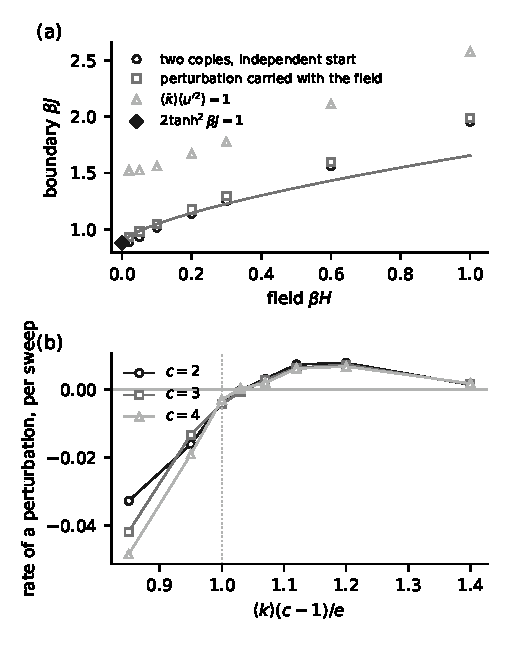
\includegraphics[width=0.66\linewidth]{figs/fig-endogeny.pdf}
\caption{\textbf{The endogeny test.} (a) The $\pm J$ spin glass on a
random regular graph of degree three in a field: the three boundaries in
$\beta J$ bisected at each field. Circles, two copies started from
independent draws of the fixed-point law stop converging; squares, a
perturbation carried alongside the field stops decaying; triangles, the
annealed criterion $\ave{\kbar}\ave{u'^{2}}=1$. The diamond is the exact
zero-field transition and the line is $\beta J_{c}+0.78\,H^{2/3}$ fitted to
the three smallest fields. (b) The hitting set on Poisson hypergraphs of
cardinality two, three and four: the stationary rate of a perturbation, per
sweep, against the mean chy-degree in units of the hard-field line
$\ave{k}(c-1)=e$ of Eq.~\eqref{eq:kc}. The three cardinalities fall on one
curve and cross zero at $1.03$ to $1.04$. Past the crossing a growing
perturbation saturates within the window, so the values there are lower
bounds on the growth rate and the points beyond $1.2$ are not drawn.
Populations of $10^{5}$;
\code{statmech/\allowbreak probe/\allowbreak endogeny.\allowbreak py} and
\code{figs/\allowbreak endogeny.\allowbreak py}.}
\label{fig:endogeny}
\end{figure}

\paragraph{The hitting set.} Chapter~\ref{ch:hittingset} had two criteria
for where its replica-symmetric answer stops being trustworthy, and they
disagree: the hard-field line $\ave{k}(c-1)=e$ of Eq.~\eqref{eq:kc}, which
is the instability of the warning map, and the soft-field entropy of
Eq.~\eqref{eq:sgen}, which on vertex cover is still positive at
$\ave{k}=3$ where the hard-field line has been crossed at $e$.
Figure~\ref{fig:endogeny}b and Table~\ref{tab:endogeny} run the test on
the soft-field population of Sec.~\ref{sec:soft} itself, at $\mu=60$, for
Poisson hypergraphs of cardinality two, three and four. Near
the boundary the perturbation's decay slows to a crawl, so the rate is
read from long stationary windows and the two halves of the window are
checked against each other; measured that way it does not move with the
chemical potential between $30$ and $120$ nor with the damping. The pair
started from independent draws has to be read with the same patience. At
the hard-field line itself it is still $10^{-2}$, $4\times10^{-3}$ and
$2\times10^{-3}$ apart after $600$ sweeps for the three cardinalities,
which a budget of $600$ sweeps and a threshold of $10^{-2}$, the
spin-glass reading, would call a boundary at or below the line; after
$2000$ sweeps it is $8\times10^{-6}$, $4\times10^{-5}$ and
$4\times10^{-5}$ and still falling at $0.003$ to $0.006$ per sweep, so
the pair converges there and the slowness is the approach to the
boundary, not the boundary. Beyond it the pair settles at a
size-independent plateau, a fifth of the pairs differing by more than
one at $\ave{k}=2.9$ on vertex cover, at $5\times10^{4}$, $2\times10^{5}$
and $4\times10^{5}$ elements alike. The rate crosses zero at $1.034$,
$1.040$ and $1.029$ times the hard-field line for the three
cardinalities, which is $\ave{k}=2.81$ against $e=2.72$ for vertex
cover. The entropy at the crossing is positive on two of the three,
$0.086\pm0.024$ and $0.038\pm0.013$, and consistent with zero on vertex
cover, $0.11\pm0.08$, where the estimator is noisiest. So the two criteria
are sorted as far as they can be: the endogeny of the soft-field solution
is lost within four per cent of the hard-field line, and the entropy has
not turned negative there, which is what a sufficient and not necessary
criterion does, as Sec.~\ref{sec:hsrsb} said and could not weigh. That the three cardinalities collapse on one curve in the
variable $\ave{k}(c-1)/e$ is Eq.~\eqref{eq:kc}'s claim that the
hard-field line is the one thing the cardinality enters through, now
measured on the soft fields.

\begin{table}[tb]
\centering\small
\begin{adjustbox}{max width=\linewidth}
% generated by figs/endogeny.py; do not edit
\begin{tabular}{lrrrr}
\hline\hline
Poisson, cardinality $c$ & hard-field line & endogeny boundary & ratio & entropy there\\
\hline
$c=2$ & 2.718 & 2.810 & 1.034 & $+0.108$\\
$c=3$ & 1.359 & 1.413 & 1.040 & $+0.086$\\
$c=4$ & 0.906 & 0.932 & 1.029 & $+0.038$\\
\hline
regular, $L$ complexes of $K$ & entropy & pair distance & rate & \\
\hline
$L=2$, $K=3$ & $+0.096$ & $0$ & $-0.0995$ & \\
$L=3$, $K=3$ & $-0.174$ & $0.81$ & $+0.0837$ & \\
$L=4$, $K=3$ & $-0.445$ & $1.03$ & $+0.0900$ & \\
$L=2$, $K=4$ & $+0.131$ & $1.2\times10^{-12}$ & $-0.1449$ & \\
$L=3$, $K=4$ & $-0.085$ & $0$ & $-0.0614$ & \\
$L=2$, $K=6$ & $+0.147$ & $4.5\times10^{-13}$ & $-0.1890$ & \\
$L=3$, $K=6$ & $-0.005$ & $1.1\times10^{-11}$ & $-0.1242$ & \\
$L=4$, $K=6$ & $-0.157$ & $2.2\times10^{-11}$ & $-0.0757$ & \\
\hline\hline
\end{tabular}

\end{adjustbox}
\caption{\textbf{Endogeny against the two criteria of
Chapter~\ref{ch:hittingset}.} Top: Poisson hypergraphs; the hard-field line
of Eq.~\eqref{eq:kc}, the zero of the stationary perturbation rate, their
ratio, and the entropy of Eq.~\eqref{eq:sgen} at the zero. Bottom: the
regular hypergraphs of \citet{mezard2007}, $L$ complexes of cardinality $K$
at every atom, where the entropy is exact: the distance between two copies
started from independent draws after $600$ sweeps, and the rate of a small
perturbation. A negative entropy proves the replica-symmetric answer wrong;
a converging pair says the fixed point is nonetheless endogenous.
\code{figs/\allowbreak endogeny.\allowbreak py}.}
\label{tab:endogeny}
\end{table}

\paragraph{Endogenous and wrong.} The bottom of Table~\ref{tab:endogeny}
is the finding the test was not run for. On the regular hypergraphs the
entropy is exact, Eq.~\eqref{eq:entropy}, and negative on five of the eight
cases, which proves the replica-symmetric answer wrong on those five. At
cardinality three the pair does not converge on either of them, the
distance staying at $0.8$ and $1.0$ with a perturbation growing at
$0.08$ per sweep: non-endogenous and wrong, the two signals together. At
cardinalities four and six the three cases with negative entropy have a
pair that converges to the last digit and a perturbation decaying at
$0.06$ to $0.12$ per sweep: the fixed point is a function of the tree
below it, and it is not the physical measure. Endogeny is a property of a
solution of the recursive distributional equation, and a wrong solution
can have it. What the contrast says is which kind of transition each case
sits past. Where endogeny is lost at the boundary --- cardinality three
here, vertex cover and the Poisson hypergraphs above --- the transition
is continuous and the linearised test finds it; where the answer is wrong
with endogeny intact, the physical measure has moved to a different
solution while the replica-symmetric one is still stable, which is the
discontinuous case of the Outlook's second pitfall, and no test on the
replica-symmetric fixed point alone can see it. The entropy can, because
it counts; the one-step calculation Sec.~\ref{sec:hsrsb} declines to do is
what would say where.

\section{What it gives the book}
\label{sec:rde-gives}

Three things, in the order the chapter reached them.

\emph{A language in which replica symmetry and its breaking are theorems
rather than ans\"atze.} Endogeny is what the replica-symmetric solution
asserts, and its failure is where Sec.~\ref{sec:onestep} begins. The book
has treated the number of fields a message carries as a choice justified
after the fact by an entropy going negative (Chapter~\ref{ch:hittingset})
or a stability line being crossed (Chapter~\ref{ch:ising}); in the
probabilistic language the choice is a property of the solution, with a
definition, and the two signals are two of its consequences.

\emph{A criterion, run.} Bivariate uniqueness,
Eq.~\eqref{eq:rde-bivariate}, is a population dynamics with two entries
per element, and Sec.~\ref{sec:rde-computed} runs it on the spin glass and
on the hitting set problem of Chapter~\ref{ch:hittingset}, where the
entropy criterion and the hard-field line are the two tests the book has
and they do not coincide. The third test, the one with a theorem behind it,
part~(c) of \citeauthor{aldous2005}'s Theorem~11, sides with the
hard-field line to within four per cent at three cardinalities, and shows
on the regular hypergraphs that a replica-symmetric answer can be
endogenous and wrong, which is the discontinuous case and the reason the
entropy is still needed.

\emph{A target statement.} That the chygraph equation is the recursive
distributional equation of the multitype branching process that is the
local weak limit of the layered ensemble, with the threshold tensor as its
mean matrix, is what a probabilist would need to be told before extending
\citet{dembo2013} from factor graphs to nested complexes; and
Sec.~\ref{sec:rde-local} says which two features of the limit --- the self
channel and the marked edge --- the extension would have to handle.

\section{What the field could get}
\label{sec:rde-field}

The survey's equations are opaque maps, and its results are results about
maps in general. The chygraph offers a class in which the map has a
structure, and the structure localises the hard questions.

First, the split. Convolution preserves the diagonal of the bivariate
recursion, so a failure of endogeny can come only from the interior
operator, and at the linear level it is decided by the kernel derivative
alone: Sec.~\ref{sec:rde-endogeny}'s identification of the de
Almeida--Thouless tensor with linearised bivariate uniqueness is a
statement about every equation of the class at once, not a computation on
one model. A criterion statable for a family, with the four moment
matrices and the two kernel derivatives $u'$ and $\hat u'$ as its only
inputs, is what the class supplies at the trivial fixed point; away from
it, Sec.~\ref{sec:rde-computed} shows, the derivative has to be carried
with the field it acts on, and the criterion is a growth rate rather than
a moment.

Second, the limit object. The local weak limit of a nested ensemble is a
multitype branching process with a self channel, a type whose offspring
includes the complex's own state feeding its members; and compound
complexes give it marked edges. The objective method has been applied to
graphs and to hypergraphs; a limit whose vertices have a state of their own
that the messages pass through is a different object, and
\citet{dembo2013}'s argument does not cover it. Stating what it is, which
Sec.~\ref{sec:rde-local} does, is the first step toward the theorem, and
the chygraph equation is the recursion that theorem would have to prove
exact.

Third, the affine case. Chapter~\ref{ch:localization} puts the Anderson
mobility edge on a clustered graph inside the classification of
\citet{alsmeyer2012}, with weights that are Schur complements and a
kernel whose symmetry is broken by the triangles. The smoothing transform
has been studied with weights that are independent of one another; the
weights of Eq.~\eqref{eq:imlinear} on a triangle are not, since the two
members of the same complex share the interior matrix, and what the
classification says about correlated weights within a bounded arity is a
question the book's ensembles pose in a concrete form.

\section{Checks}
\label{sec:rde-checks}

\checkhead{Known results}
\code{statmech/\allowbreak probe/\allowbreak endogeny.\allowbreak py}
bisects, on the $\pm J$ spin glass of degree three, three boundaries at
seven fields between $0.02$ and $1$, and
\code{figs/\allowbreak endogeny.\allowbreak py} checks, before it draws,
that the linearised boundary approaches the exact zero-field transition
$2\tanh^{2}\beta J=1$ as $\beta J_{c}+aH^{2/3}$ with residuals below
$0.03$, and that the pair boundary lies within eight per cent of it.
\code{statmech/\allowbreak tests/\allowbreak test\_\allowbreak
endogeny.\allowbreak py} pins that identical copies stay identical to the
last bit, that the zero-field transition is where it should be, that a
perturbation decays below the line and the pair fails to converge deep in
the glass, and that on vertex cover the pair converges at $\ave{k}=2$ and
does not at $4$.

\checkhead{New results}
The endogeny boundary of the soft-field hitting set at three
cardinalities against the hard-field line and the entropy, and the
regular cases of Table~\ref{tab:endogeny}. The rate is read from
stationary windows of $600$ sweeps at damping one half, its two halves
agreeing to $0.001$ per sweep near the boundary; the boundary is
unchanged at chemical potentials $30$, $60$ and $120$ and at damping
$0.2$; the plateau of a non-converging pair is unchanged between
$5\times10^{4}$ and $4\times10^{5}$ elements; and the pair at and below
the hard-field line is followed to $2000$ sweeps, where it is still
converging.

\checkhead{Partial results}
The pair boundary of the spin glass is bisected on a fixed budget of
$600$ sweeps and a threshold of $10^{-2}$, and reads two to five per cent
below the linearised one for that reason; it is not a separate
determination of the line. The entropy on Poisson ensembles carries the
scatter Sec.~\ref{sec:hs-checks} describes, $0.07$ on vertex cover, and
one estimate near $e$ overflowed and is left out. The scan takes about
seventy minutes and is cached; nothing in the chapter recomputes it.
